해당 장에서는 이번 프로젝트를 진행하면서 사용한 메소드에 대해 설명한다.
프로젝트의 주제인 슈퍼 마리오 게임 특성상 게임 화면을 통해 내용이 전개된다. 
따라서 우리는 \ref{sec:survey:DQN}에서 설명한 DQN 메소드를 기본으로 사용한다.
기존 발표된 기법 중 하나인 Deep Q-Network(DQN) 메소드에 추가적인 화면 분할을 통해 여러 구역을 학습하는 Split DQN을 설명하고, 최종적으로 Split DQN에 Attention 개념을 추가한 Split Attention DQN 메소드에 대해 설명한다.

위에서 간략히 설명한 제안 메소드를 설명하기에 앞서 이 게임에서 강화학습에 필요한 state, action, 그리고 reward를 어떻게 얻어내는지에 대해 하위 섹션~\ref{sec:method:basis}에서 다룬다.
섹션~\ref{sec:method:idea}에서는 Split DQN과 Split Attention DQN에 대해 소개한다.

\subsection{강화학습 기본 요소 추출}
\label{sec:method:basis}
강화학습에서 현재 state는 이 후 action을 결정하는 데 중요한 요소이다.
실제 게임 플레이어와 공평한 조건에서 경쟁하기 위해 본 프로젝트에서 state를 화면에 표시되는 이미지를 사용하여 결정하기로 하였다.
Convolutaionl neural network (CNN)~\cite{CNN}은 이미지로 부터 학습 모델에 필요한 feature를 추출하여 의사 결정에 활용하는 널리 알려진 방법이다.
본 프로젝트에서 우리는 화면 이미지를 CNN을 통해 해석하여 게임 점수를 최대한 얻을 수 있는 action을 추론하는 모델을 만들고자 한다.

우리는 키 조합을 통해 action을 생성할 수 있는데 유의미한 조합만을 고려하면 Table~\ref{tab:mario:action}과 같은 16개의 action을 정의할 수 있다.
여기서 유의미한 조합이라 함은, 무의미한 조합을 제외한 키 조합을 의미한다.
슈퍼 마리오는 총 6개의 키를 가지고 있으므로 총 64개의 키 조합을 가지는 데, 이 중 left + right와 같이 서로 상반되는 동작을 동시에 지정하는 경우에는 게임 내부의 키 매핑에 의해 아무 행동을 하지 않게 된다.
이러한 무의미한 action의 경우 우리의 학습 모델에 혼동만 주기 때문에 미리 제외하였다.
%
\begin{table}[h]
	\caption {
		슈퍼 마리오 브라더스에서 가능한 키 입력 조합. 가능한 조합 중 유의미한 키 조합만을 선별하였다.
	}
	\label{tab:mario:action}
\centering	
\begin{tabular}{lcccccc}
\toprule
          & Left & Right & Up & Down & A & B \\
\midrule
Action 1  &      &       &    &      &   &   \\
Action 2  & *    &       &    &      &   &   \\
Action 3  &      & *     &    &      &   &   \\
Action 4  &      &       & *  &      &   &   \\
Action 5  &      &       &    & *    &   &   \\
Action 6  &      &       &    &      & * &   \\
Action 7  &      &       &    &      &   & * \\
Action 8  &      &       &    &      & * & * \\
Action 9  & *    &       &    &      & * &   \\
Action 10 & *    &       &    &      &   & * \\
Action 11 & *    &       &    &      & * & * \\
Action 12 &      & *     &    &      & * &   \\
Action 13 &      & *     &    &      &   & * \\
Action 14 &      & *     &    &      & * & * \\
Action 15 &      &       & *  &      &   & * \\
Action 16 &      &       &    & *    &   & * \\
\bottomrule
\end{tabular}
\end{table}
%
우리의 모델은 최종적으로 Figure~\ref{fig:overview}와 같이 현재 state에서 각 차원이 각 action에 대응되는 16차원의 vector를 산출하여 각 action의 적합성을 확률적으로 추론한다.
\begin{figure}[]
\begin{center}
\begin{tabular}{c}
     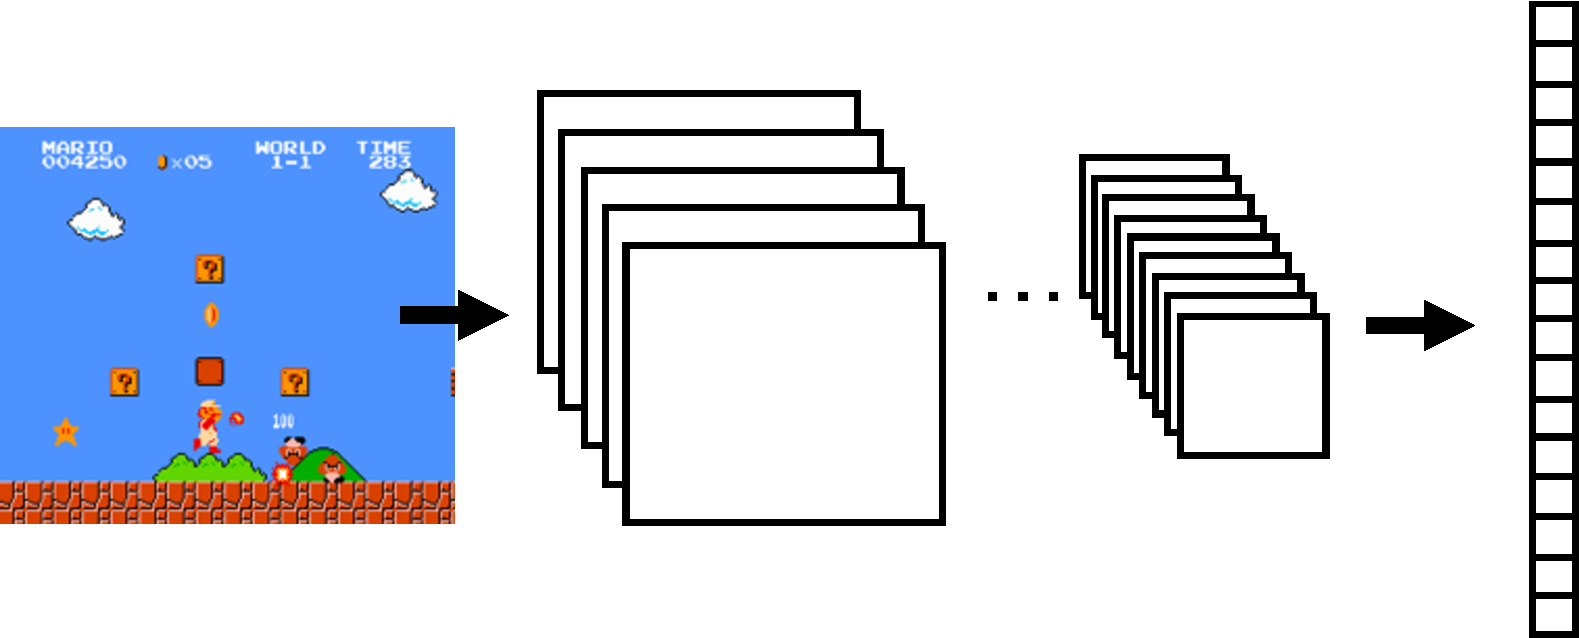
\includegraphics[width=0.4\textwidth]{FIG/overview.pdf} \\
\end{tabular}
\caption{
	게임 화면으로부터 action을 추론하기 위한 모델. CNN을 통해 게임화면을 해석하여 16차원의 action의 적합성을 추론한다.
}
\label{fig:overview}
\end{center}
\end{figure}

강화학습에서 모델은 현재 state에서 최종적으로 얻을 수 있는 reward를 극대화하는 action을 선택하도록 학습된다.
따라서 reward를 잘 설정해야 올바른 선택을 하도록 유도할 수 있다.
슈퍼 마리오 브라더스 게임에서 stage가 끝날 때 남은 시간당 50점을 획득하게 된다.
이는 다른 방법으로 얻는 점수보다 상당히 많은 양이다.
이번 프로젝트에서 해결하려는 것은 마리오를 가능한 빠른 시간 안에 목적지까지 도착하게 하는 것이다. 
따라서 획득 점수 위주로 reward를 설정하였을 때, 마리오가 빠른 시간안에 깃발로 도달하도록 유도할 수 있다.




이러한 방법 외에도 마리오의 이동 위치에 따라 추가적으로 reward를 제공하는 방법을 사용하였다. 
이러한 방법을 사용하는 이유는 마리오가 깃발에 가까워질수록 reward가 더 커지는 것을 인지하게 하려함이다. 
여러 시도 끝에 마리오가 목적지 방향인 오른쪽 방향으로 이동을 하였을 때 보상을 받고, 왼쪽 방향으로 이동을 하였을 때 패널티를 받는다면 마리오는 오른쪽 방향으로 이동하는 것이 보상을 받는다는 것을 인지하고, 왼쪽보다는 오른쪽으로 이동하려 할 것이다.
오른쪽 방향으로 이동함에 따라 reward를 제공하며 에이전트에게 골 라인으로 도달하는 가이드라인을 주는 효과를 볼 수 있다.
Reward를 제공하는 방식은 다음과 같다.
만약 마리오가 이전 위치보다 좌측으로 n만큼 이동하였다면 이는 목적지에서 더욱 멀어지는 방향으로 가고 있다 판단되어 -5만큼의 reward를 제공한다. 
반대로 만약 마리오가 이전 위치보다 우측으로 n만큼 이동하였다면 이는 목적지와 가까운 방향으로 이동하고 있고 목적지로 달성한다고 판단되어 +5만큼의 reward를 제공한다.
여기에 추가로 만약 마리오가 이전 위치에서 움직이지 않는다면 -1만큼의 reward를 제공함으로써 마리오를 목적지 방향으로 움직이려는 시도를 한다. 

위와 같은 reward를 제공하는 방법과 더불어 시간이 지남에 따라 패널티를 제공한다. 
한 스테이지가 시작되면 제한 시간이 존재한다. 
제한 시간안에 목적지에 도달하지 못하면 게임은 끝이 나는데, 제한 시간에 패널티를 제공하는 방식이다. 
시간이 1초가 지날 때마다 -1의 리워드를 제공하여 빠른 시간 안에 목적지에 도달할 수 있도록 구현하였다. 

% 삭제 해야하나영
또한, stage 중간에 코인, 아이템, 그리고 적을 처치해서 얻는 점수를 고려하면 중간중간의 imediate reward로 활용되어 마리오가 해당 동작을 하도록 하는 학습을 할 수 있다.
이와 같이, stage 내부의 획득 점수를 통해 reward를 주는 것은 올바른 게임 플레이를 학습하는 데 도움을 준다.

게임의 특성상 마리오를 큰 마리오, 나아가 슈퍼 마리오로 변신시키면 남은 stage를 진행함에 있어 크게 유리한 요소로 작용한다.
우리 모델이 슈퍼 마리오로 변신하는 것을 지향하고 변신이 풀리는 것을 지양하기 위해 상위 단계로 변신할 때 획득 점수이외의 부가적인 reward를 할당하고, 변신이 풀릴 경우 reward를 크게 감소시키도록 한다.

\subsection{DQN}
\label{sec:method:dqn}
DQN 설명

\subsection{Split DQN (\sdqnname)}
\label{sec:method:sdqn}
S-DQN 설명

\subsection{Split Attention DQN (\sadqnname)}
\label{sec:method:idea}
사람들이 슈퍼 마리오 브라더스를 실제로 플레이할 때, 사람들은 상황에 따라 화면의 일부분을 좀 더 집중해서 바라보게 된다.
예를 들면, 마리오가 공중에서 하강하고 있을 때는 마리오의 아래 쪽에 집중하여 바닥의 함정을 피하거나 적을 밟아 처치하도록 조작한다.
전반적으로, 전체 화면의 내용보다 마리오 주변에서 일어나고 있는 일에 집중하는 경향이 있다.

\begin{figure}[]
\begin{center}
\begin{tabular}{c}
     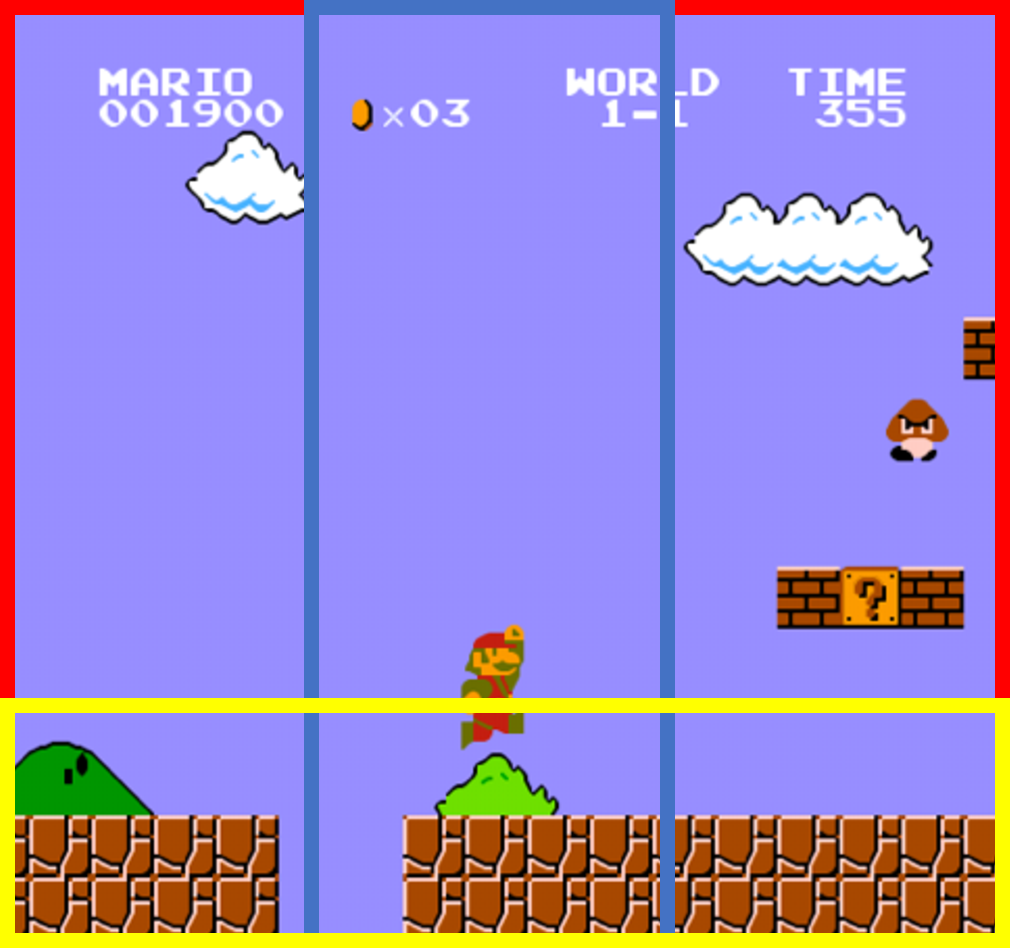
\includegraphics[width=0.4\textwidth]{FIG/split_screen.pdf} \\
\end{tabular}
\caption{
	화면 분할을 통해 여러 CNN 입력을 생성하는 예시. 전체 화면을 나타내는 빨간색, 마리오 주변을 나타내는 파란색, 그리고 바닥의 함정을 조심하기 위한 노란색 영역이 있다.
}
\label{fig:split_screen}
\end{center}
\end{figure}

이러한 게임의 특성을 고려하여 우리 모델도 여러 개의 CNN을 만들어 화면의 각 구역별로 따로 feature를 추출하기로 한다.
이렇게 추출한 feature의 중요도는 마리오의 상황에 따라 변화한다. 앞서 예와 같이 마리오가 공중에 있다면 마리오 주변에 좀 더 집중해야 한다.
만약 마리오의 달리기 속도가 빠른 상황이라면 좀 더 전체 화면부위를 고려하여 다음 action을 정해야한다.
또한 바닥의 함정에 빠지면 마리오가 즉사할 수 있으므로 아래 쪽 영역에 대한 주의도 늦출 수 없다.
우리 모델에서는 figure~\ref{fig:split_screen}과 같이 여러 구역으로 나눠 입력을 만든 후 각각의 CNN으로 생성된 feature를 마리오의 현재 상황에 따라 중요도를 계산하도록 Attention~\cite{Attention}을 통해 현재 feature를 결정하도록 한다.

그림에서 보는 바와 같이 빨간색 구역은 전체 화면을 포함한다. 
파란색 구역은 마리오를 중심으로 하는 세로 크기의 구역을 포함하는데 이는 마리오 주변의 상황을 확인하기 위함이다.
마지막으로 노란색 구역은 화면 아래를 포함한다. 
따라서 노란색 구역은 땅, 적, 구멍과 같은 부분을 집중한다. 

Split DQN을 처리하는 과정은 Figure \ref{fig:split_dqn}와 같다. 
각각 분할된 구역에 대해 Convolutional Neural Network 과정을 거친다. 
결과적으로 width와 height의 크기가 8X8의 통일된 크기를 가진다. 
여기서 다른 부분은 바로 채널의 크기인데, 전체 화면을 처리하는 빨간색 영역에 대해서는 최종적으로 48개의 채널을 가진다.
이와 다르게 나머지 파란색 구역과 노란색 구역에 대한 처리는 최종적으로 각각 24개의 채널을 가진다. 
이렇게 총 세 개의 결과물을 합치는 과정을 거치는데 이때 Concatenate 연산을 통해 최종적으로 8X8X96 크기를 가진 매트릭스를 출력한다. 
이러한 결과를 Softmax 연산을 통해 총 16개의 액션을 의미하는 벡터를 출력한 뒤 가장 값이 높은 action을 선택한다. 

% 검토 필요합니답
Split Attention DQN은 여기에 각각의 채널에 대해 weight sum을 하여 어느 곳에 더 큰 비중을 줄지를 결정해 더 나은 결정을 할 수 있도록 유도한다. 


\begin{figure}[]
\begin{center}
\begin{tabular}{c}
     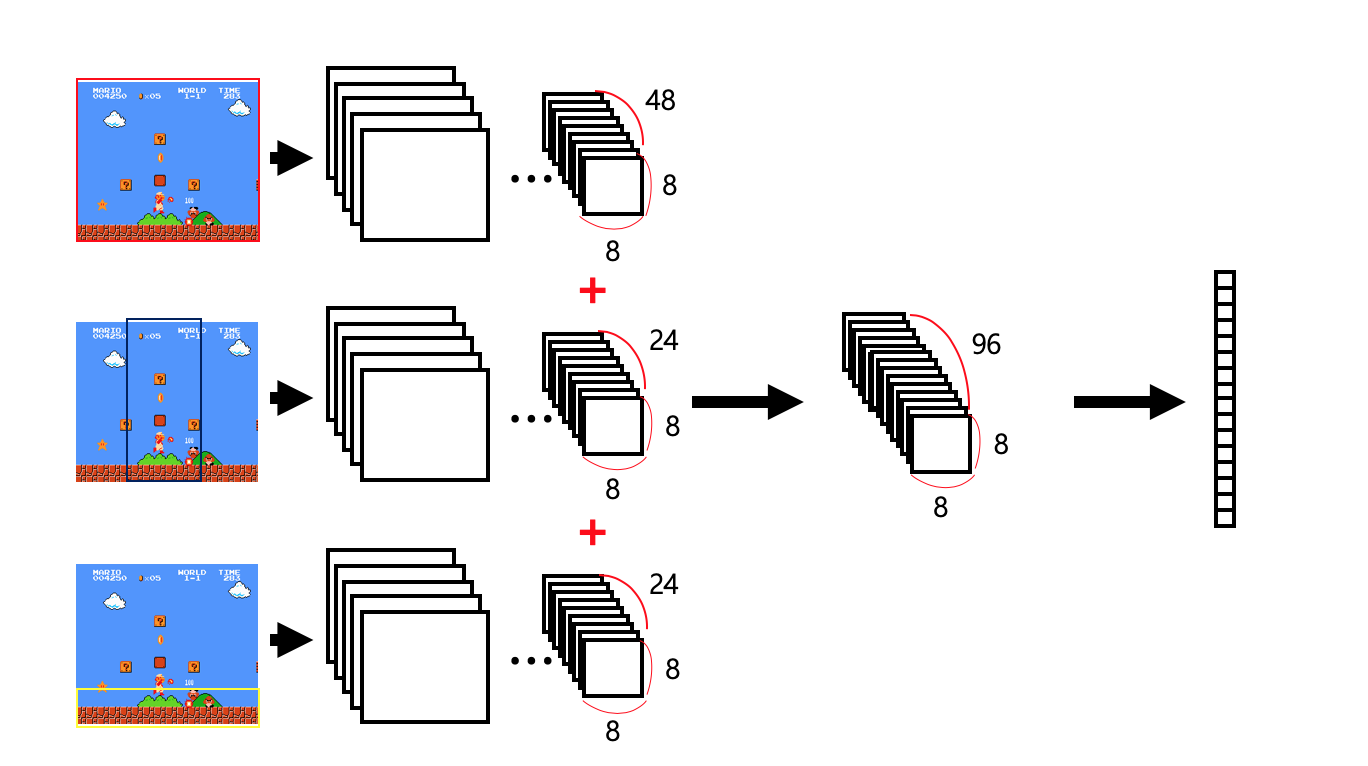
\includegraphics[width=0.8\textwidth]{FIG/split_dqn.png} \\
\end{tabular}
\caption{
	Split DQN의 CNN 처리 방식
}
\label{fig:split_dqn}
\end{center}
\end{figure}

